\documentclass{llncs}
\usepackage{graphicx}
\usepackage[portuguese]{babel}
\usepackage[utf8]{inputenc}
\usepackage{fullpage}
\usepackage{indentfirst}
\usepackage{colortbl} % Permite o uso de cores em tabelas
\usepackage{url}
 
\renewcommand{\labelitemi}{$\bullet$}

\renewenvironment{quote}{%
  \list{}{%
    \leftmargin3.0cm   % this is the adjusting screw
    \rightmargin\leftmargin
  }
  \item\relax
}
{\endlist}

\begin{document}

\begin{figure}[!t]
\centering 

\includegraphics[width=15.5cm]{images/logo.pdf}
\end{figure}

\title{Aplicação de programação orientada à organização de agentes no Multi-Agent Programming Contest}
\author{Mariana Ramos Franco e Rafael Barbolo Lopes}
% \institute{Escola Politécnica da Universidade de São Paulo \\ Departamento de Engenharia de Computação e Sistemas Digitais \\ PCS 5703 - Sistemas Multi-Agentes}
\institute{PCS 5703 - Sistemas Multi-Agentes}
\date{21 de Maio de 2011}

\maketitle

\begin{abstract}
Este trabalho apresenta o projeto e implementação de um SMA para participação no \textit{Agent Contest} através da aplicação de programação orientada à organização de agentes. Para isso utilizou-se o modelo organizacional MOISE+ e a plataforma JASON.
\end{abstract}

% ### INTRODUÇÃO ###
\section{Introdução}

% Breve descrição do problema, bem como de software (modelos, plataformas, etc) e hardware utilizados.

O objetivo do trabalho é projetar e implementar um Sistema Multi-Agente (SMA) para participar do \textit{Agent Contest} de 2009.

O \textit{Multi-Agent Programming Contest} é uma competição em que simultaneamente, dois times são situados no mesmo ambiente e competem diretamente num cenário definido pelos organizadores. Por se tratar de uma competição direta, é um cenário interessante para avaliar e comparar diferentes sistemas, assim possibilitando identificar pontos fortes e fracos de cada sistema, promovendo e avaliando o desenvolvimento de todos os participantes.

Conforme citado em \cite{AC}, o \textit{Multi-Agent Programming Contest} tem as seguintes características:

\begin{quote}
\textit{"This competition is an attempt to stimulate research in the area of multiagent systems development and programming by:}
\begin{enumerate}
\item \textit{Identifying key problems,}
\item \textit{Collecting suitable benchmarks, and}
\item \textit{Gathering test cases which require and enforce coordinated action that can serve as milestones for testing multi-agent programming languages, platforms and tools."}
\end{enumerate}
\end{quote}

Em 2009, o \textit{Agent Contest} definiu como tema para a competição um cenário de pastoreio, em que os agentes (comboys) estão localizados em um grid com árvores, vacas, cercas, currais e botões (que permitem a abertura da cerca). Árvores e currais são elementos estáticos, enquanto as cercas são controladas pelos agentes por meio de botões. Já as vacas possuem um algoritmo de movimentação com base nos elementos em torno delas, de modo a sofrerem atração mútua (tendendo a se agrupar) e a serem repelitas pelos obstáculos e agentes. A intensidade de cada um desses parâmetros comportamentais pode variar para cada cenário e é definida pelos organizadores do \textit{Agent Contest}, não estando disponível diretamente para os competidores.


% ### ANÁLISE E ESPECIFICAÇÃO DO SMA ###
\section{Análise e Especificação do SMA}

% Descrição do método adotado para o desenvolvimento do SMA; especificação dos requisitos do SMA e especificação dos componentes do SMA (agentes, organização, interações, etc) segundo o método de desenvolvimento adotado.

% \begin{enumerate}
%  \item How is your system  specified and designed?
%  \item Did you use any existing multi-agent system methodology such as Prometheus, Gaia or Tropos?
%  \item Which strategies and algorithms do you plan to use?
%  \item How are the following agent features implemented: 
% 			\emph{autonomy}, \emph{proactiveness} and \emph{communication} 
%			\emph{team working}, and \emph{coordination}?
%  \item Is your system a truly \textbf{multi}-agent system or rather a centralised system in disguise?
% \end{enumerate}

Para o desenvolvimento do SMA foi utilizado um método situacional construido sob medida para o projeto, a partir de fragmentos de métodos capturados de três abordagens de desenvolvimento: USDP \cite{USDP}, Gaia \cite{GAIA} e MOISE+ \cite{MOISE}.

O método é composto de quatro fases situacionais: Especificação de Requisitos, Análise, Design e Implementação.

Na fase de Especificação de Requisitos foram definidos os atores e os casos de uso do sistema. Já a fase de Análise foi composta de três subfases: Descrição do Ambiente em Gaia, Descrição da Organização em MOISE+, e Descrição das Interações usando Gaia.


% ### ESPECIFICAÇÃO DE REQUISITOS ###
\subsection{Especificação de Requisitos}


% ### IDENTIFICAÇÃO DOS ATORES ###
\subsubsection{Identificação dos Atores}

\begin{center}
\begin{tabular}{|l|p{3cm}|p{8cm}|}
\hline
\rowcolor[gray]{0.8} \textbf{Ator}	&\textbf{Papel}	&\textbf{Uso do sistema} \\
\hline
cowboy	&Capturar vacas		&Move-se pelo pasto, interage com vacas, abre/fecha cerca, interage com cowboy líder \\ 
\hline
cowboy sabotador	&Atrapalhar equipe adversária	&Move-se pelo pasto, interage com vacas, abre/fecha cerca da outra equipe, interage com cowboy líder \\
\hline
cowboy líder	&Coordenar cowboys	&Move-se pelo pasto, interage com vacas, abre/fecha cerca, coordena cowboys \\
\hline
vaca	&Pastar	&Move-se pelo pasto, se aproxima de rebanhos, se afasta de cowboys e de obstáculos \\
\hline
\end{tabular}
\end{center}

\textit{Observação: o ator vaca é implementado pelo simulador e por isso casos de uso iniciados por ele não serão apresentados neste documento.}


% ### IDENTIFICAÇÃO DOS CASOS DE USO ###
\subsubsection{Identificação dos Casos de Uso}

\begin{center}
\begin{tabular}{|p{3cm}|p{10cm}|}
\hline
\rowcolor[gray]{0.8} \textbf{Caso de uso}		&\textbf{Breve descrição} \\
\hline
Procurar vaca	&Cowboys movem-se pelo pasto até encontrar uma vaca \\
\hline
Capturar vaca	&Ao encontrar uma vaca, cowboys organizam-se para capturá-la \\
\hline
Atrapalhar equipe adversária &O cowboy sabotador atrapalha a equipe adversária \\
\hline
Abrir/fechar cerca	&Cowboy se aproxima (ou se afasta) do botão para abrir (ou fechar) a cerca  \\
\hline
\end{tabular}
\end{center}


% ### DESCRIÇÃO DOS CASOS DE USO ###
\subsubsection{Descrição dos Casos de Uso}

% Caso de Uso: Procurar vaca
\begin{center}
\begin{tabular}{|p{2.5cm}|p{10cm}|}
\hline
\rowcolor[gray]{0.8} \textbf{Caso de Uso:}	&\textbf{Procurar vaca} \\
\hline
\textbf{Ator:} 			&cowboy, cowboy líder, vaca. \\
\hline
\textbf{Início:}		&Cowboy líder deseja encontrar uma vaca. \\
\hline
\end{tabular}
\begin{tabular}{|p{0.5cm}|p{12cm}|}
\hline
\multicolumn{2}{|c|}{\textbf{Fluxo Típico}} \\
\hline
\textbf{No}	&\textbf{Ação} \\
\hline
1	&Cowboys e comboy líder movimentam-se para uma nova posição. \\
\hline
2	&Cowboy encontra uma vaca na vizinhança. \\
\hline
3	&Cowboy grava o identificador e a coordenada da vaca encontrada. \\
\hline
\multicolumn{2}{|c|}{\textbf{Fluxos Alternativos}} \\
\hline
\multicolumn{2}{|l|}{\textbf{Alternativa 1:} Nenhum cowboy encontrou vaca no movimento.} \\
\hline
\textbf{No}	&\textbf{Ação} \\
\hline
2	&Cowboy não encontra uma vaca na vizinhança. \\
\hline
3	&Repete passo 1. \\
\hline
\end{tabular}
\end{center}

% Caso de Uso: Capturar vaca
\begin{center}
\begin{tabular}{|p{2.5cm}|p{10cm}|}
\hline
\rowcolor[gray]{0.8} \textbf{Caso de Uso:}	&\textbf{Capturar vaca} \\
\hline
\textbf{Ator:} 			&cowboy, cowboy líder, vaca. \\
\hline
\textbf{Início:}		&Cowboy encontrou uma vaca. \\
\hline
\end{tabular}
\begin{tabular}{|p{0.5cm}|p{12cm}|}
\hline
\multicolumn{2}{|c|}{\textbf{Fluxo Típico}} \\
\hline
\textbf{No}	&\textbf{Ação} \\
\hline
1	&Cowboy emite o identificador e a coordenada da vaca para o cowboy líder. \\
\hline
2	&Cowboy líder emite ordem de captura com identificador e coordenada da vaca para todos os cowboys. \\
\hline
3	&Cowboys fazem formação um ao lado do outro para empurrar a vaca para a cerca (cowboy líder comanda o movimento). \\
\hline
4	&Cowboys encurralam vaca na cerca. \\
\hline
5	&Cowboy líder manda o cowboy mais próximo do botão abrir a cerca. \\
\hline
6	&Vaca entra na cerca. \\
\hline
7	&Cowboy fecha a cerca. \\
\hline
8	&Cowboys desfazem formação. \\
\hline
\end{tabular}
\end{center}

% Caso de Uso: Atrapalhar equipe adversária
\begin{center}
\begin{tabular}{|p{2.5cm}|p{10cm}|}
\hline
\rowcolor[gray]{0.8} \textbf{Caso de Uso:}	&\textbf{Atrapalhar equipe adversária} \\
\hline
\textbf{Ator:} 			&cowboy sabotador. \\
\hline
\textbf{Início:}		&Cowboy sabotador caminha até a cerca do adversário. \\
\hline
\end{tabular}
\begin{tabular}{|p{0.5cm}|p{12cm}|}
\hline
\multicolumn{2}{|c|}{\textbf{Fluxo Típico}} \\
\hline
\textbf{No}	&\textbf{Ação} \\
\hline
1	&Cowboy sabotador chega na cerca do adversário. \\
\hline
2	&Cowboy sabotador envia estímulos para o botão da cerca para mantê-la sempre aberta. \\
\hline
\end{tabular}
\end{center}


% ### DIAGRAMA DO MODELO DE CASOS DE USO ###
\subsubsection{Diagrama do Modelo de Casos de Uso}

\paragraph{ }

\begin{figure}[!ht]
\centering 
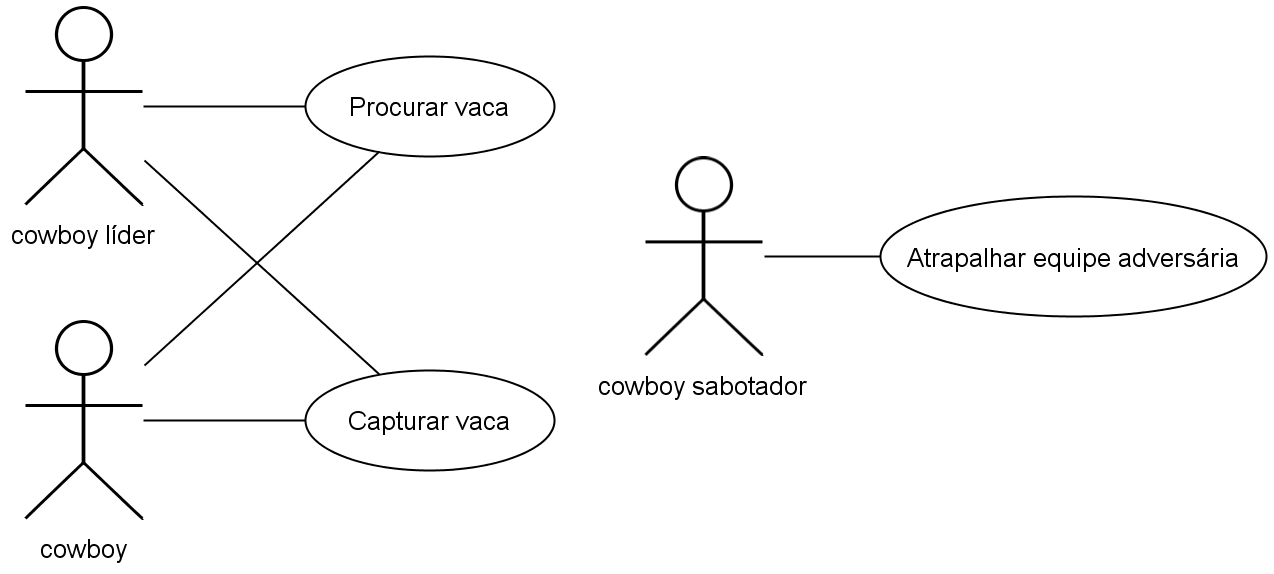
\includegraphics[width=15cm]{images/usecase.png}
\caption{Diagrama do Modelo de Casos de Uso}
\end{figure}

% ### ANÁLISE DO SMA ###
\subsection{Análise do SMA}


% ### DESCRIÇÃO DO AMBIENTE ###
\subsubsection{Descrição do Ambiente (Gaia)}

\paragraph{ }
O ambiente em que o SMA atuará é composto de uma grade de células. O tamanho da grade é especificado no início da simulação e é variável. Porém, ele não pode ter mais de 150 x 150 células. A coordenada [0, 0] da grade está no canto superior esquerdo (noroeste). O ambiente simulado possui dois currais retangulares – um para cada equipe – que servem como um local para onde as vacas devem ser dirigidas. Além disso, há cercas que podem ser abertas através de botões.

Cada célula da grade pode ser ocupada por exatamente um dos seguintes objetos:

\begin{itemize}
\item Agente (controlado e capaz de se mover de uma célula para outra adjacente);
\item Obstáculo (bloqueia a célula);
\item Vaca (controlada pelo simulador, pode se mover de uma célula para outra adjacente, tende a formar rebanhos em áreas abertas e mantém distância de obstáculos e de agentes);
\item Cerca (pode ser aberta usando um botão, para isto o agente deve ficar parado na célula adjacente ao respectivo botão).
\end{itemize}

Vacas devem ser empurradas para os currais. Cada time aprende a posição e as dimensões do seu curral no início de cada simulação.

\begin{figure}[!ht]
\centering 
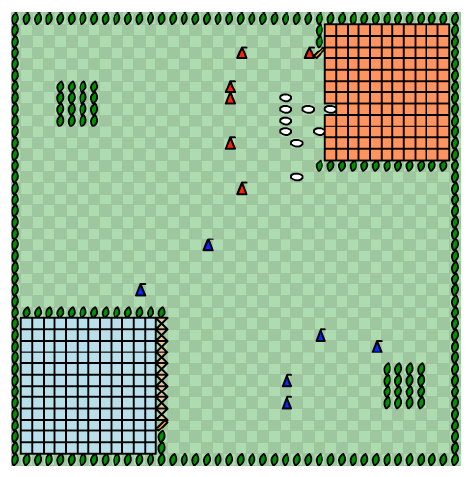
\includegraphics[width=10cm]{images/env.png}
\caption{Ambiente de simulação. Agentes (triângulos vermelhos e azuis) são dirigidos pelos competidores. Obstáculos (círculos verde) bloqueiam células. Vacas (círculos brancos) movimentam-se de acordo com um algoritmo de vaca. Cercas (formas em x) podem ser abertas por um agente parado na célula adjacente ao botão (em forma de barra). As vacas têm que ser empurradas para dentro dos currais (retângulos vermelhos e azuis.)}
\end{figure}


% ### DESCRIÇÃO DA ORGANIZAÇÃO ###
\subsubsection{Descrição da Organização (MOISE+)}

\paragraph{ }
O propósito da organização de agentes é capturar o maior número possível de vacas e atrapalhar o time adversário.

Existem 3 grupos de agentes:

\begin{itemize}
\item Liderança: grupo composto pelo cowboy líder que coordena os outros cowboys;
\item Sabotagem: grupo composto pelo cowboy sabotador que procura atrapalhar a equipe adversária;
\item Captura: grupo composto pelos cowboys responsáveis por capturar as vacas.
\end{itemize}

Existem 3 metas a serem cumpridas pelos agentes: procurar vaca, capturar vaca e atrapalhar equipe adversária. Para cada uma dessas metas, há missões específicas que os agentes devem cumprir. A especificação funcional no item 3.1 apresenta essas metas e missões.


% ### DESCRIÇÃO DAS INTERAÇÕES ###
\subsubsection{Descrição das Interações (Gaia)}

\paragraph{ }
O modelo de interações representa as dependências e relacionamentos entre os papéis do sistema multiagentes, de acordo com as definições de um protocolo de comunicação entre os agentes.

As comunicações entre os agentes modelados ocorrem apenas entre os agentes com papel de capturador e o agente com papel de coordenador. Mais detalhes são dados no item 3.2.


% ### ARQUITETURA E DESIGN DO SMA ###
\section{Arquitetura e Design do SMA}

% Design dos componentes do SMA e descrição da arquitetura do SMA, segundo o método de desenvolvimento adotado.

% \begin{enumerate}
%  \item Which programming language do you plan to use to implement the multi-agent system?
%  \item How would you map the designed architecture (both multi-agent and individual agent architectures)
%    to programming codes, i.e., how would you implement specific agent-oriented
%    concepts and designed artifacts using the programming language?
%  \item Which development platform, tools and techniques are you planning to use?
% \end{enumerate}
% Please give reasons why you have chosen the methods explained above.

A fase de design (projeto) do SMA especificada no método situacional é composta de quatro subfases: Modelo de Organização (MOISE+), Modelo de Interações (Gaia), Projeto de Agentes (Gaia) e Projeto de Comportamento Organizacional (MOISE+).


% ### MODELO DE ORGANIZAÇÃO (MOISE+) ###
\subsection{Modelo de Organização (MOISE+)}

MOISE+ define 3 tipos de especificação para o modelo e projeto de organizações em um SMA: 

\begin{itemize}
\item Especificação Estrutural: define os papéis, relações entre papéis e grupos.
\item Especificação Funcional: define as missões e planos.
\item Especificação Deôntica: especifica, no nível individual, como permissões e obrigações de um papél estão relacionas com uma missão.
\end{itemize}


\newpage
% ### ESPECIFICAÇÃO ESTRUTURAL ###
\subsubsection{Especificação Estrutural}

\paragraph{ }

\begin{figure}[!ht]
\centering 
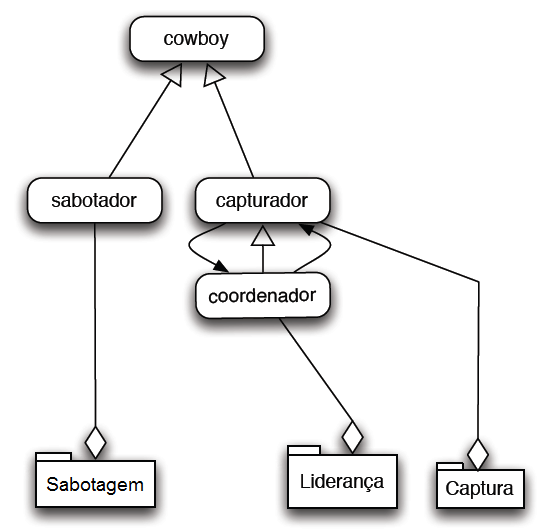
\includegraphics[width=8cm]{images/structuraspec.png}
\caption{Especificação Estrutural}
\end{figure}

\begin{center}
\begin{tabular}{|l|l|l|}
\hline
\rowcolor[gray]{0.8} \textbf{Papel de origem}		&\textbf{Papel de destino} 	& \textbf{Tipo de link}\\
\hline
Coordenador	&Capturador	&Autoridade \\
\hline
Capturador	&Coordenador	&Comunicação \\
\hline
\end{tabular}
\\ Links entre papéis
\end{center}

\newpage

% ### ESPECIFICAÇÃO FUNCIONAL ###
\subsubsection{Especificação Funcional}

\paragraph{ }

\begin{figure}[!ht]
\centering 
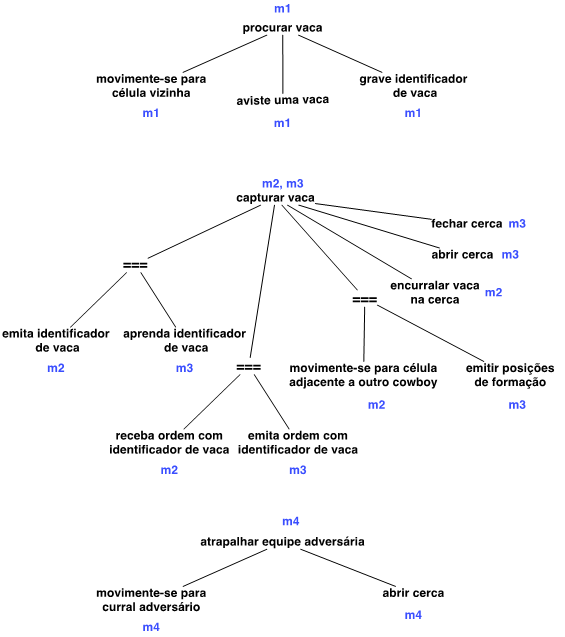
\includegraphics[width=11cm]{images/functionalspec.png}
\caption{Especificação Estrutural}
\end{figure}


% ### ESPECIFICAÇÃO DEÔNTICA ###
\subsubsection{Especificação Deôntica}

\begin{center}
\begin{tabular}{|l|l|l|l|}
\hline
\rowcolor[gray]{0.8} \textbf{Papel}		&\textbf{Relação deôntica} 	&\textbf{Missão}	&\textbf{Restrição temporal}\\
\hline
Sabotador	&Obrigação	&m4	&A qualquer momento \\
\hline
Capturador	&Obrigação	&m1	&Enquanto procura vaca \\
\hline
Capturador	&Obrigação	&m2	&Enquanto captura vaca \\
\hline
Coordenador	&Obrigação	&m1	&Enquanto captura vaca \\
\hline
\end{tabular}
\end{center}

\newpage

% ### MODELO DE INTERAÇÕES (GAIA) ###
\subsection{Modelo de Interações (Gaia)}

As comunicações entre os agentes modelados ocorrem apenas entre os agentes com papel de capturador e o agente com papel de coordenador.

A seguir definimos os possíveis protocolos de comunicação entre os agentes:


% Protocolo: Encontrou vaca
\begin{center}
\begin{tabular}{|p{2.5cm}|p{2.5cm}|p{5cm}}
\cline{1-2}
\multicolumn{2}{|l|}{Protocolo:} \\
\multicolumn{2}{|l|}{Encontrou vaca}  \\
\hline
Iniciador: 			&Parceiro:		&Entrada: \\
comboy 			&cowboy líder		&identificador e coordenada da vaca encontrada. \\
\hline
\multicolumn{2}{|p{5cm}|}{Descrição:}  &Saída \\
\multicolumn{2}{|p{5cm}|}{Comboy informa o líder que encontrou uma vaca.}  &OK, dados recebidos. \\
\hline
\end{tabular}
\end{center}

% Protocolo: Cercar vaca
\begin{center}
\begin{tabular}{|p{2.5cm}|p{2.5cm}|p{5cm}}
\cline{1-2}
\multicolumn{2}{|l|}{Protocolo:} \\
\multicolumn{2}{|l|}{Cercar vaca}  \\
\hline
Iniciador: 			&Parceiro:		&Entrada: \\
cowboy líder 			&cowboy		&identificador e coordenada da vaca a ser capturada; coordenada para onde o cowboy deve se locomover para começar a cercar a vaca. \\
\hline
\multicolumn{2}{|p{5cm}|}{Descrição:}  &Saída \\
\multicolumn{2}{|p{5cm}|}{Líder ordena o cowboy capturar vaca.}  &OK, dados recebidos. \\
\hline
\end{tabular}
\end{center}

% Protocolo: Abrir/Fechar cerca
\begin{center}
\begin{tabular}{|p{2.5cm}|p{2.5cm}|p{5cm}}
\cline{1-2}
\multicolumn{2}{|l|}{Protocolo:} \\
\multicolumn{2}{|l|}{Abrir/Fechar cerca}  \\
\hline
Iniciador: 			&Parceiro:		&Entrada: \\
cowboy líder 			&cowboy		&vaca no curral.\\
\hline
\multicolumn{2}{|p{5cm}|}{Descrição:}  &Saída \\
\multicolumn{2}{|p{5cm}|}{Líder ordena o cowboy a abrir/fechar a cerca.}  &OK, cerca aberta/fechada. \\
\hline
\end{tabular}
\end{center}


% ### PROJETO DE AGENTES (GAIA) ###
\subsection{Projeto de Agentes (Gaia)}

O time de agentes para a competição será sempre formado de:

\begin{itemize}
\item 1 comboy líder
\item 1 comboy sabotador
\item 1 à N comboys
\end{itemize}

onde N é o número máximo de agentes no time - 2.

% ### PROJETO DO COMPORTAMENTO ORGANIZACIONAL DOS AGENTES ###
\subsection{Projeto de Comportamento Organizacional (MOISE+)}

No sistema multiagente proposto, não é possível que agentes entrem ou saiam do ambiente. Cada time é composto de um número fixo (definido pelo simulador) de cowboys que permanecem no ambiente durante toda a simulação.

Os agentes recebem os papéis no início da simulação. Um agente receberá o papel de coordenador, e liderará a procura e captura de vacas. Outro agente receberá o papel de sabotador, e terá como missão atrapalhar o time adversário a atingir seus objetivos. Os outros agentes serão capturadores, e agirão em conjunto na procura e captura de vacas.

Todos os agentes do sistema estão compromissados com pelo menos uma meta global do sistema(capturar vacas e atrapalhar o adversário). As metas locais desses agentes foram projetadas para alcançar as metas globais. Logo, o comportamento dos agentes sempre será dirigido por missões locais que visam as metas globais.


% ### LINGUAGENS DE PROGRAMAÇÃO E PLATAFORMA DE EXECUÇÃO ###
\section{Linguagens de programação e plataforma de execução}

% Tecnologia SMA utilizada, características da implementação, etc.

Para o desenvolvimento do SMA, foram utilizadas as linguagens XML, Java e AgentSpeak. Para executar o SMA, foi utilizado o interpretador Jason. Como ambiente de desenvolvimento, foi utilizada a IDE Eclipse com o plugin Jason instalado. A seguir, cada uma dessas tecnologias será apresentada com seu papel no projeto.

A linguagem de marcação XML foi utilizada para definir a especificação organizacional do SMA em MOISE+. Foram descritas as especificações estrutural, funcional e normativa do SMA em XML.

A linguagem Java foi utilizada para implementar o socket de comunicação com o servidor de simulação do \textit{Multi-Agent Programming Contest} de 2009, assim como para implementar muitas das funcionalidades dos agentes. Por exemplo, a funcionalidade de movimento de um agente foi implementada em Java, através de cálculo de rota e troca de mensagens com o servidor de simulação.

A linguagem AgentSpeak foi utilizada para implementar os agentes. Para cada agente, foram definidas suas crenças, regras e metas iniciais, assim como as missões às quais ele estaria comprometido em realizar. Também foram implementados eventos organizacionais, estruturais e funcionais para cada agente, assim como seus planos, utilizando a linguagem AgentSpeak.

O interpretador Jason foi utilizado para executar e depurar o SMA desenvolvido. Ele realiza a conexão entre a organização MOISE+ definida em XML, as implementações dos agentes em AgentSpeak e as implementações de suas funcionalidades em Java. Para facilitar o desenvolvimento, foi utilizada a IDE Eclipse com o plugin Jason instalado.


% ### ESTRATÉGIA PARA TIME DE AGENTES ###
\section{Estratégia para time de agentes}

% Descrição do algoritmo de deslocamento dos agentes, das estratégias de coordenação e de otimização de tarefas, etc.

% \begin{enumerate}
%    \item Describe the navigation algorithms:
%        \begin{itemize}
%            \item obstacle avoiding
%            \item strategy for finding and herding cows
%            \item opponent blocking
%        \end{itemize}
%    \item Describe the team coordination strategy (if any)
%    \item Does your team strategy use some distributed optimization
%        technique w.r.t. e.g.  minimizing distances walked by the
%        agents?
%    \item Describe and discuss the information exchanged (and shared) in
%        the agent team.
%    \item Describe the communication strategy in the agent team. Can you
%        estimate the communication complexity in your approach?
%    \item Did your system do some background processing? Under background
%        processing we understand some computation which happened while agents of
%        the team were \textit{idle}, i.e. between sending an action
%        message to the simulation server and receiving a perception
%        message for the subsequent simulation step.
%    \item Possibly discuss additional technical details of your system like
%        e.g. failure/crash recovery and alike.
% \end{enumerate}

A estratégia do nosso time de agentes consiste em:

\begin{itemize}
\item Capturar pelo menos 1 vaca durante a partida;
\item Impedir que o time adversário capture vacas.
\end{itemize}

Para garantir a captura de pelo menos 1 vaca, foi implementado um esquema de captura de vacas que consiste em procurar uma vaca e guardá-la dentro da cerca. Para impedir que o time adversário capture vacas, foi implementado um esquema que garante que a cerca do adversário esteja sempre aberta, tornando-se impossível guardar a vaca dentro da cerca.

% TODO: Describe what is stored in the word model

O algoritmo de deslocamento de agentes implementado consiste em receber a posição atual do agente e a posição final desejada. Com isso, é possível obter o sentido de movimento que deve ser percorrido (\textit{norte}, \textit{nordeste}, \textit{leste}, \textit{sudeste}, \textit{sul}, \textit{sudoeste}, \textit{oeste} ou \textit{noroeste}). Antes de executar o movimento, é verificado se não há um obstáculo na posição que será alcançada. Quando há obstáculo, o agente se move aleatoriamente em outro sentido, sem que ocorra bloqueio de seu movimento.


% TODO: Herding cows (check if the text below is fine)

A procura de uma vaca consiste em um agente \textit{cowboy} se movimentar pelo ambiente até sentir a presença de uma vaca. Após encontrar a vaca, o agente informa ao agente \textit{cowboy líder} a localização desta vaca e sua captura é iniciada. A captura de uma vaca é feita em grupo pelos agentes \textit{cowboys}. O \textit{cowboy líder} envia a localização da vaca para os outros \textit{cowboys}, que a encurralam e a empurram em sentido à cerca. Quando a vaca chega próxima à cerca, o \textit{cowboy líder} abre a cerca e os \textit{cowboys} empurram a vaca para dentro dela. Quando a vaca entra na cerca, o \textit{cowboy líder} simplesmente a fecha.

Para impedir que o time adversário capture vacas, um cowboy \textit{sabotador} se move até a cerca do time adversário e a mantém sempre aberta. Desta forma, é improvável que uma vaca capturada da equipe adversária ficará presa dentro da cerca.

% ### CARACTERÍSTICAS TÉCNICAS ###
\section{Características técnicas}

% Descrição de características técnicas do SMA desenvolvido, tais como estabilidade e recuperação de falhas.

O sistema desenvolvido apresentou instabilidade de comunicação com o servidor de simulação, pois este aguarda um \textit{timeout} (tempo de resposta) grande antes de executar as ações dos agentes em um único passo. Desta forma, alguns agentes enviam uma sequência de mensagens que nem sempre são recebidas pelo servidor de simulação, o que gera ciclos de processamento em inanição.

Testamos a situação em que a simulação é interrompida e o nosso sistema reinicia a partir do ponto que parou. Alguns problemas foram observados neste caso. Cada agente do SMA possui uma representação do mundo, que é construída no decorrer da simulação. Ao interromper a simulação, todo o conhecimento de mundo acumulado é destruído (pois este está armazenado em memória dinâmica). Ao reiniciar a simulação em um ponto diferente, é comum que os agentes levem um certo tempo até aprenderem novamente as informações do mundo e darem continuidade à execução de seus objetivos de forma coordenada.

Foi observado que o sistema consome uma baixa quantidade de memória, porém uma elevada taxa de processamento. A baixa quantidade memória ocorre porque as estruturas de dados armazenam informações muito simples, como pequenas cadeias de caracteres e inteiros. A elevada taxa de processamento ocorre porque o servidor de comunicação não é em tempo real, o que faz com que muitos ciclos com trocas de mensagem sejam cancelados.

% ### DISCUSSÃO E CONCLUSÃO ###
\section{Discussão e conclusão}

% Comentários sobre a facilidade/dificuldade de utilização do método de desenvolvimento adotado, comentários sobre a facilidade e ou dificuldade do modelo organizacional para este domínio, bem como possíveis extensões que poderiam ser realizadas na solução proposta.

% In this section please expand a bit on your experience with the
% contest organization, the proposed scenario, and the setup of the
% actual contest. Please indicate what do you see as pros/cons of
% participating in the Contest with respect to your research in the
% field.
% \begin{enumerate}
%    \item Critical discussion of your approach to the development of the
%        agent team.
%    \item Will you gain some insights/experiences into developing multi-agent system in
%        the course of participating in the Agent Contest so far? If so,
%        what kind of?
%    \item Do you think that the Agent Contest can serve its
%        purpose to provide a testbed for state-of-the-art multi-agent
%        systems development frameworks?
%    \item Describe and discuss possible problems that you face in choosing approach, programming
%        platform or technical infrastructure to participate in this contest?
%\end{enumerate}

O método situacional adotado mostrou-se muito completo nas fases de análise, especificação e design. Através das atividades propostas, foi possível especificar muito bem o SMA e construir corretamente os modelos propostos na fase de design. Na fase de implementação, o método situacional forneceu uma sequência lógica de atividades que contribuiu para a implementação dos agentes e do ambiente. Exceto por esta última fase, todas as outras foram seguidas, atividade por atividade, durante o desenvolvimento do SMA.

O modelo organizacional baseado em MOISE+ foi muito bem aplicado ao domínio do SMA. Não houve dificuldade em mapear as estruturas e funcionalidades do SMA para o modelo organizacional adotado. A implementação da organização também foi fácil utilizando Jason.

% TODO: Discuss cows herding

Através das simulações de execução do nosso time de agentes, verificamos que a sabotagem da equipe adversária funciona bem tecnicamente. É necessário verificar se esta estratégia funcionará bem em uma competição real. Para melhorar a sabotagem da equipe adversária, seria interessante criar mais agentes que atrapalham o processo de captura de vacas da equipe adversária (por exemplo, agentes que empurram as vacas no sentido contrário à entrada da cerca).

Houve dificuldade em encontrar recursos online para aprendizado de programação de SMA usando Jason. Os artigos online eram muito simples e a documentação da API de Jason para Java era complexa. Para a disseminação de tecnologias multiagentes, seria interessante o desenvolvimento de recursos online de aprendizado mais acessíveis, principalmente para plataformas mais populares, como Jason.

Com o desenvolvimento do projeto para o \textit{Multi-Agent Programming Contest}, ganhamos experiência com a plataforma Jason, que, apesar de complexa, se mostrou muito poderosa e flexível para a programação de SMAs. O projeto contribuiu muito com o entendimento de como são realizadas interações entre os diversos agentes de um SMA, ficando claro que não é possível controlar sequências de ações de um grupo de agentes ou mesmo de um único agente. Também foi muito útil para obter experiência prática com organização de agentes utilizando MOISE+.

\bibliographystyle{plain}
\bibliography{myrefs}

\end{document}

